% This must be in the first 5 lines to tell arXiv to use pdfLaTeX, which is strongly recommended.
\pdfoutput=1
% In particular, the hyperref package requires pdfLaTeX in order to break URLs across lines.

\documentclass[11pt]{article}

% Remove the ``guidelines`` option to generate the final version.
%\usepackage[guidelines]{nlpreport} % show guidelines
\usepackage[]{nlpreport} % hide guidelines


% Standard package includes
\usepackage{times}
\usepackage{latexsym}

% For proper rendering and hyphenation of words containing Latin characters (including in bib files)
\usepackage[T1]{fontenc}
% For Vietnamese characters
% \usepackage[T5]{fontenc}
% See https://www.latex-project.org/help/documentation/encguide.pdf for other character sets

% This assumes your files are encoded as UTF8
\usepackage[utf8]{inputenc}

% This is not strictly necessary, and may be commented out,
% but it will improve the layout of the manuscript,
% and will typically save some space.
\usepackage{microtype}
\usepackage{graphicx}
\usepackage{rotating}
\usepackage{hyperref}
\usepackage{amsmath}
\usepackage{mathtools}
\usepackage{multirow}
\usepackage{listings}
\usepackage{xcolor}
\usepackage{booktabs} % for tables
\usepackage{float}






% THE pdfinfo Title AND Author ARE NOT NECESSARY, THEY ARE METADATA FOR THE FINAL PDF FILE
\hypersetup{pdfinfo={
Title={Human Value Detection: a brief summary of simple neural network and transformer architectures},
Author={Vincenzo Collura, Gianmarco Pappacoda, Anthea Silvia Sasdelli\\}
}}
%\setcounter{secnumdepth}{0}  
 \begin{document}
%
\title{Human Value Detection: a brief summary of simple neural network and transformer architectures\\
}
\author{Vincenzo Collura,
Gianmarco Pappacoda,
\and
Anthea Silvia Sasdelli\\
Master's Degree in Artificial Intelligence, University of Bologna\\
\{ vincenzo.collura2, gianmarco.pappacoda, anthea.sasdelli \}@studio.unibo.it
}
\maketitle


\attention{DO NOT MODIFY THIS TEMPLATE - EXCEPT, OF COURSE FOR TITLE, SUBTITLE AND AUTHORS.\\ IN THE FINAL VERSION, IN THE \LaTeX\ SOURCE REMOVE THE \texttt{guidelines} OPTION FROM  \texttt{$\backslash$usepackage[guidelines]\{nlpreport\}}.
}

\begin{abstract}
%\begin{quote}
Human values are ``trans-situational goals(...) that serve as guiding principles in the life of a person or group''\cite{Schwartz2012}. Therefore, humans tend to express natural language arguments guided by underlying values which are dependent on a number of factors such as the cultural context and transcend situations.
The purpose of the challenge proposed by \cite{Kiesel2022} is: given a textual argument and a human value category, to classify whether or not the argument draws on the Schwartz categories\cite{Schwartz2012} of human values.
The authors of this report propose a number of neural architectures to be evaluated for the task. Furthermore, the proposed architectures include ``simpler'' neural architectures as well as more complex ones, so-called ``large language models'' powered by the underlying architecture known as ``transformers''.

\explanation{
The abstract is very brief summary of your report. Try to keep it no longer than 15-20 lines at most. Write your objective, your approach, and your main observations (what are the findings that make this report worthwhile reading?)
}

%\end{quote}
\end{abstract}

\attention{\textcolor{red}{NOTICE: THIS REPORT'S LENGTH MUST RESPECT THE FOLLOWING PAGE LIMITS: \begin{itemize}
    \item ASSIGNMENT: \textbf{2 PAGES} 
    \item NLP PROJECT OR PROJECT WORK: \textbf{8 PAGES}
    \item COMBINED NLP PROJECT + PW: \textbf{12 PAGES}
\end{itemize}  PLUS LINKS, REFERENCES AND APPENDICES.\\ 
THIS MEANS THAT YOU CANNOT FILL ALL SECTIONS TO MAXIMUM LENGTH. IT ALSO MEANS THAT, QUITE POSSIBLY, YOU WILL HAVE TO LEAVE OUT OF THE REPORT PART OF THE WORK YOU HAVE DONE OR OBSERVATIONS YOU HAVE. THIS IS NORMAL: THE REPORT SHOULD EMPHASIZE WHAT IS MOST SIGNIFICANT, NOTEWORTHY, AND REFER TO THE NOTEBOOK FOR ANYTHING ELSE.\\ 
FOR ANY OTHER ASPECT OF YOUR WORK THAT YOU WOULD LIKE TO EMPHASIZE BUT CANNOT EXPLAIN HERE FOR LACK OF SPACE, FEEL FREE TO ADD COMMENTS IN THE NOTEBOOK.\\ 
INTERESTING TEXT EXAMPLES THAT EXCEED THE MAXIMUM LENGTH OF THE REPORT CAN BE PLACED IN A DEDICATED APPENDIX AFTER THE REFERENCES.}}


\section{Introduction}
\label{sec:introduction}
\attention{MAX 1 COLUMN FOR ASSIGNMENT REPORTS / 2 COLUMNS FOR PROJECT OR PW / 3 FOR COMBINED REPORTS.}
As human values are underlying driving forces of humans' decisions, understanding them and being able to predict whether a human value is present or not in a given argument as such driving force is an important feat.
Being able to rightly classify the speech values of an interlocutor can be very useful but also very complex.
As a matter of fact, the sheer amount of emotions that populate the emotional spectrum of humans makes this operation very difficult.

The challenge proposed by \cite{Kiesel2022} is: given a textual argument expressed in natural language and a human value decide whether or not the textual argument draws from the given human value.

The problem can be easily framed as a multi-label classification one.

The provided dataset is composed of $7289$ arguments, expressed as triplets each composed of a \textit{Premise}, a \textit{Conclusion} and a \textit{Stance} (i.e. whether the conclusion is in favour of or against the premise).

\begin{figure}[H]
    \centering
    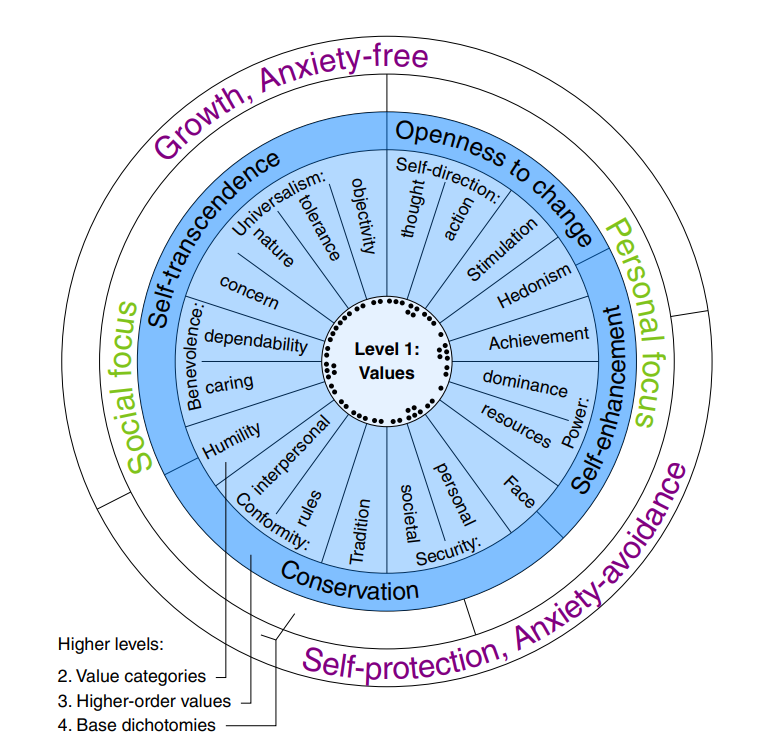
\includegraphics[width=8cm]{figures/schwartz_values.png}
    \caption{Image of the 20 value categories. Categories that tend to conflict are placed on opposite sites. Illustration adapted from \cite{Kiesel2022} and \cite{Schwartz2012}}
    \label{fig:values}
\end{figure}

Each argument is uniquely identified and is associated with 20 ``level2'' labels (a form of aggregation over ``raw'' human values).
The test dataset does not contain such labels.

This project goal is to assess the performance of ``simpler'' neural architectures in conjunction with a dense vector representation of words and more complex pre-trained large language models architectures known as ``transformers''.

GloVe\cite{Pennington2014} has been selected as dense vector representation the simpler neural architectures. Transformers-based solutions already use specific embeddings.

All the proposed solutions are trained, evaluated against validation and test sets using the metrics proposed by the paper authors (F1-score, Precision and Recall using macro average).

\explanation{
The Introduction is an executive summary, which you can think of as an extended abstract.  Start by writing a brief description of the problem you are tackling and why it is important. (Skip it if this is an assignment report).} 

\explanation{Then give a short overview of known/standard/possible approaches to that problems, if any, and what are their advantages/limitations.} 

\explanation{After that, discuss your approach, and motivate why you follow that approach. If you are drawing inspiration from an existing model, study, paper, textbook example, challenge, \dots, be sure to add all the necessary references~\cite{DBLP:journals/corr/abs-2204-02311,DBLP:conf/acl/LorenzoMN22,DBLP:conf/clef/AnticiBIIGR21,DBLP:conf/ijcai/NakovCHAEBPSM21,DBLP:conf/naacl/RottgerVHP22,DBLP:journals/toit/LippiT16}.\footnote{\href{https://en.wikipedia.org/wiki/The_Muppet_Show}{Add only what is relevant.}}}

\explanation{Next, give a brief summary of your experimental setup: how many experiments did you run on which dataset. Last, make a list of the main results or take-home lessons from your work.}

\attention{HERE AND EVERYWHERE ELSE: ALWAYS KEEP IN MIND THAT, CRUCIALLY, WHATEVER TEXT/CODE/FIGURES/IDEAS/... YOU TAKE FROM ELSEWHERE MUST BE CLEARLY IDENTIFIED AND PROPERLY REFERENCED IN THE REPORT.}

\section{Background}
\label{sec:background}
\attention{MAX 2 COLUMNS (3 FOR COMBINED REPORTS). DO NOT INCLUDE SECTION IF NO BACKGROUND NECESSARY. OMIT SECTION IN ASSIGNMENT REPORTS.}

To proceed in the analysis and the implementation of this project the \cite{Kiesel2022} paper was fundamental.
The advantage given by a customized dataset of 5270 arguments from four geographical cultures, manually annotated for human values allows to overcome the obstacle of the large variety of the human values, by accounting for many different cultural contexts and providing the survey with cultural-specific questions.

The aforementioned work is based on \cite{Schwartz2012} that establishes the cornerstones for the classes of human values to be defined. 

"The theory defines and orders 19 values on the continuum based on their compatible and conflicting motivations, expression of self-protection vs. growth, and personal vs. social focus." \cite{Schwartz2012}

Another important psychological paper concerning human values is ``The Nature of Human Values''\cite{Rokeach1976}.
He estimates the total number of human values to be fewer than hundreds, and develops a practical survey of 36 values that distinguishes between values pertaining to desirable end states and desirable behaviour.

It has been noted that in the data the premise or the conclusion can be used multiple times with different respective stances.

What happens is the reframing of the text, which means the change of perspective with respect to an issue.
In fact, it is possible that, from the same premise, the consequent conclusion captures different aspects or topics.
This is important also for the understanding of the data in the preprocessing.
This topic is developed in the paper \cite{Chen2021}


\explanation{The Background section is where you briefly provide whatever background information on the domain or challenge you're addressing and/or on the techniques/approaches you're using, that (1) you think is necessary for the reader to understand your work and design choices, and (2) is not something that has been explained to you during the NLP course (to be clear: do NOT repeat explanations of things seen in class, we already know that stuff). If you adapt paragraphs from articles, books, online resources, etc: be sure to clarify which parts are yours and which ones aren't.}

\section{System description}
\label{sec:system}
\attention{MAX 1 COLUMN FOR ASSIGNMENT REPORTS / 4 COLUMNS FOR PROJECT OR PW / 6 FOR COMBINED REPORTS.}

In order to ensure reproducibility a seed (i.e. number) has been set for all the random number generators (RNGs) involved in the process. While the authors have striven to ensure reproducibility, some employed libraries such as HuggingFace exhibited a fluctuating behaviour with respect to this issue. 

The first performed step was the download of the dataset, the arguments and the labels ones, each already splitted in train, test and validation.

As test set labels are not available unless actively participating in the challenge, the authors have decided to discard the test set and produce another test set by randomly selecting samples from the training set up to $\approx 15\%$ its size ($\approx 800$ samples).

In order to better grasp the nature and the distribution of the data, an explanatory data analysis phase has been carried out, revealing the dataset labels to be unevenly distributed (please refer to Figure \ref{fig:labels_dist}).

Another aspect that was checked is the the distribution of sentences length (accounting for the summation of premise, stance and conclusion): in training and validation sets are, as hypothesized, comparable. This ensures the validation set is employable to perform validation during training. Moreover, it is possible to cut the sequences in order to reduce the computational power needed to perform both training and inference. In order to perform the cut, the 99th percentile of the lengths has been selected. Needless to say, were the distribution of the documents sentences to change, the maximum allowed sentence length would have to be adjusted accordingly.

The system has been split into two different sections:
\begin{itemize}
\item Simpler network architectures employing dense vector representations (GloVe only)
\item Transformer-based models repurposed (i.e. fine-tuned) for the task
\end{itemize}

In both sections the training data has been preprocessed by concatenating the stance (converted to a single word: favor/against), the conclusion and the stance. The input data is then converted to lower-case.

In the first section the data is also stripped of punctuation as it could impair model training. The lower-case transformation is very important for the first section since GloVe, that is the chosen embedding method, only has lower-case mappings. This passage is fundamental in order to check and find real Out-Of-Vocabulary (OOV) words contained in the data.

%copiato dal primo report
The word embedding has been implemented as part of the neural network in the form of a neural network layer. The embedding layer depends on the building process of the embedding matrix which in turn depends on the vocabulary. During this step words whose embedding is known are translated, words whose embedding is not known (OOVs) are translated into vectors whose dimensions have a uniform distribution.
%copiato dal primo report

The first proposed architecture, ``BiLSTM'' is a simple Bidirectional LSTM layer with $36$ units, its output is passed across an average pooling and a max pooling layer in a parallel way, the output is then feed into a fully-connected layer using ReLU as activation function.

The second proposed architecture, ``CNNText'' implements a series of convolutional layers with $36$ filters and increasing sizes of kernels (1,2,3,5), no padding, $\text{stride}=1$. The input is flattened and passed into the first layer. Once passed the last layer

The aforementioned two architectures are adaptations of \cite{Agarwal2020}.

The second section describes the implementation of transformer-based solutions. The authors proposed  \texttt{BERTTiny}\cite{Bhargava2021, Turc2019} $\approx 4.5M$ parameters and \texttt{DistilRoBERTa-base}\cite{Sanh2019} ($\approx 82M$ parameters). The chosen architectures are among the smallest transformers while delivering near-SOTA performance in many tasks.

In both transformer architectures, the final part of the neural network (often referred to as ``head'') has been cut off and replaced by fully-connected layers and a dropout layer in order to repurpose the language models.


\explanation{
Describe the system or systems you have implemented (architectures, pipelines, etc), and used to run your experiments. If you reuse parts of code written by others, be sure to make very clear your original contribution in terms of
\begin{itemize}
    \item architecture: is the architecture your design or did you take it from somewhere else
    \item coding: which parts of code are original or heavily adapted? adapted from existing sources? taken from external sources with minimal adaptations?
\end{itemize}
It is a good idea to add figures to illustrate your pipeline and/or architecture(s)
(see Figure~\ref{fig:architecture})
%
\begin{figure*}
    \centering
    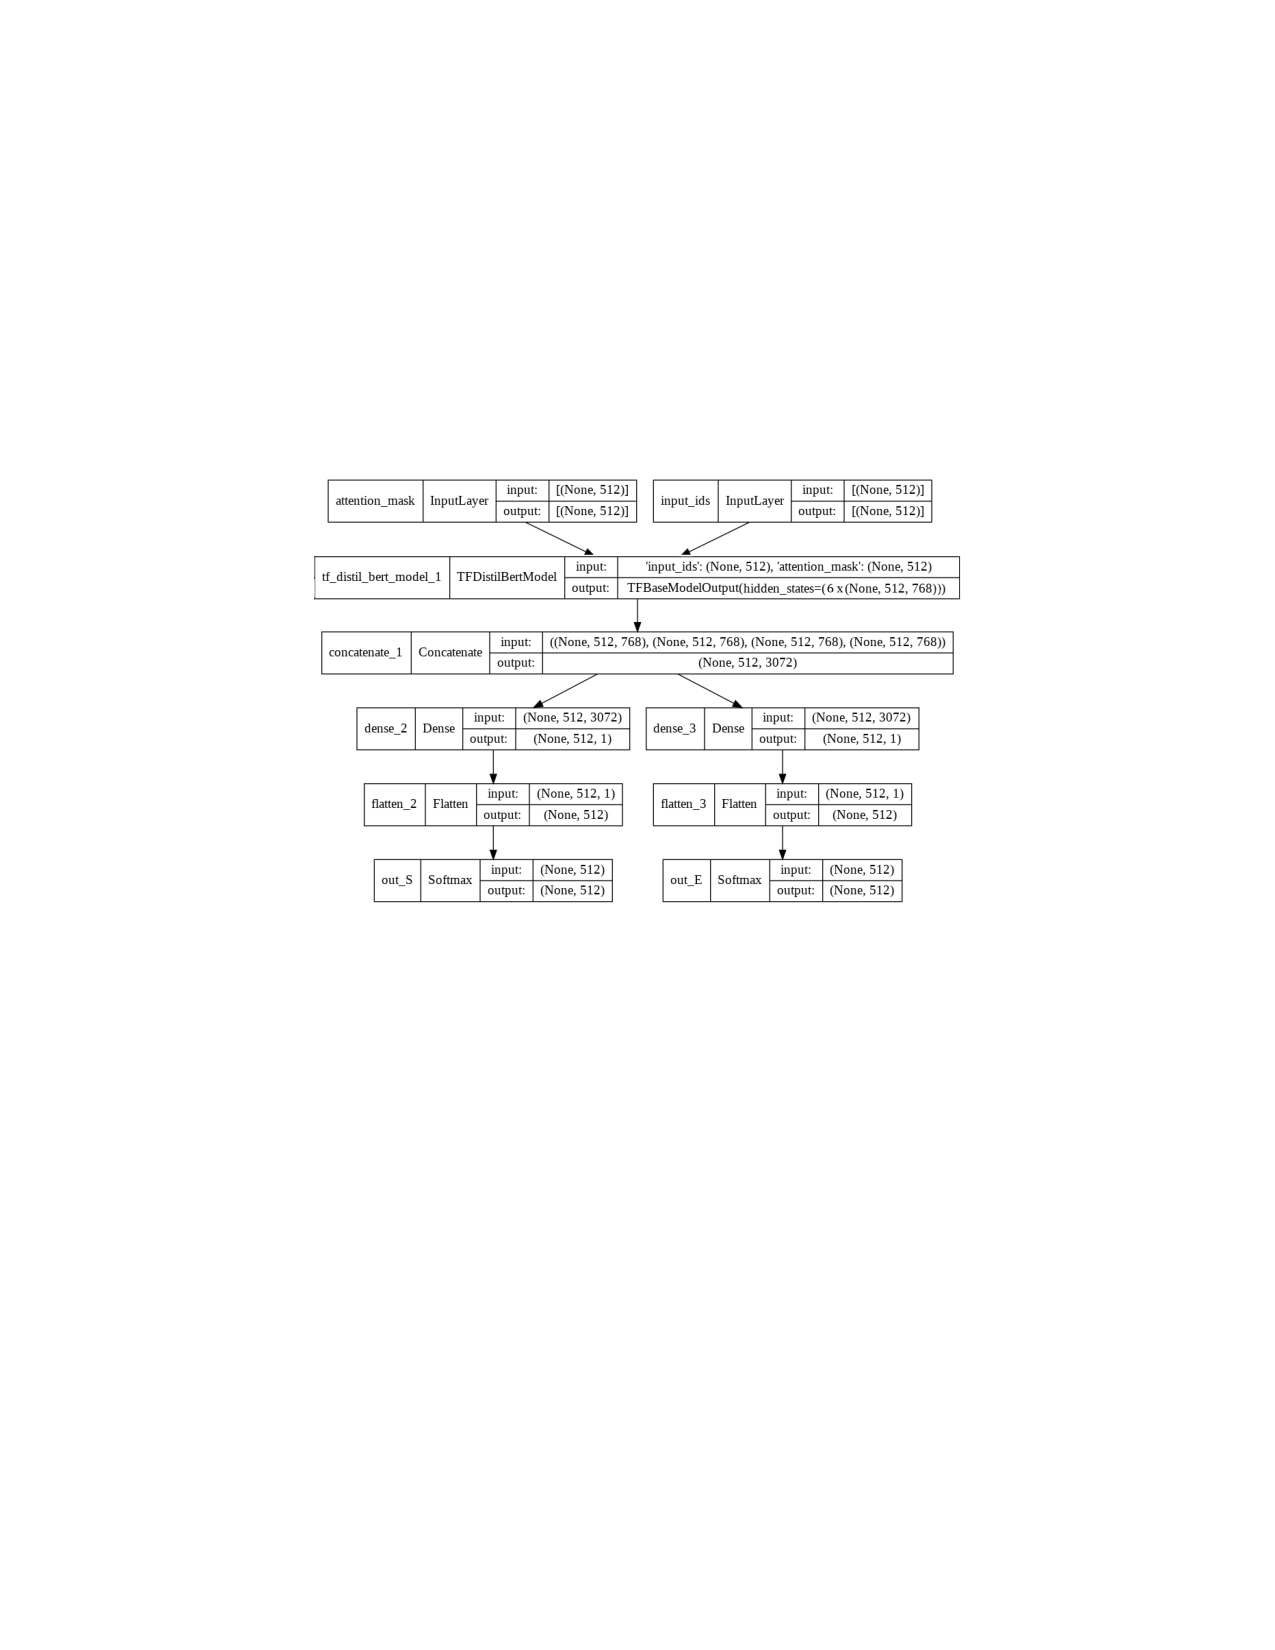
\includegraphics[width=\textwidth]{img/architecture.pdf}
    \caption{Model architecture}
    \label{fig:architecture}
\end{figure*}
}

\section{Data}
\label{sec:data}
\attention{MAX 2 COLUMNS / 3 FOR COMBINED REPORTS. OMIT SECTION IN ASSIGNMENT REPORTS.}
The dataset used for this project was provided by Touché23-Human-Value-Detection \cite{Kiesel2022}. \\
The original dataset is pre-split into training, test and validation splits, however the test split is not labelled, therefore the authors have decided to discard it in favour of a new test set obtained by randomly extracting samples from the training set up to $\approx 15\%$ of its size ($\approx 800$ samples).

The dataset is further split into two main sections, the first one containing arguments as triplets and the second one containing the labels.

Each sample in the first section is composed of

\begin{itemize}
\item the argument ID 
\item the conclusion, which is the final stance with respect to the premise.
\item the stance, which has only two values: ``in favor of'' or ``against''. It connects the conclusion and the premise by specifying whether the former is in favor of or against the latter.
\item the premise, which is a text or a sentence that gives the context, the core, of the argument.
\end{itemize}

The second section contains labels. Each sample is composed by 21 features, representing the argument ID followed by the 20 ``level2'' value categories. Each feature can either be $1$: the argument draws on that category, or $0$ the argument does not draw on that category. Categories are not mutually exclusive.

\explanation{Provide a brief description of your data including some statistics and pointers (references to articles/URLs) to be used to obtain the data. Describe any pre-processing work you did. Links to datasets must be placed later in Section~\ref{sec:links}.}

\section{Experimental setup and results}
\label{sec:results}
\attention{MAX 1 COLUMN FOR ASSIGNMENT REPORTS / 3 COLUMNS FOR PROJECT OR PW / 5 FOR COMBINED REPORTS.}

A seed has been set for all the involved frameworks as to ensure reproducibility.
To accomplish the goal of this project two variants of neural networks have been chosen: simple neural networks with dense vector representations and transformers-powered large language models.
The starting idea being to start the implementation with a simpler architecture, and then compare the results with a more complex system, such as large language models.

In the first solution the data was preprocessed, in order to check the maximum length of the sentences in the arguments datasets and the distribution of sentences length in training and validation sets.
Then the vocabulary was built, using GloVe\cite{Pennington2014} as embedding with dimension equal to 300 and always taking into account and adding the OOV words at each step (training, validation, test).

As the neural networks output are in the form of logits, a sigmoid function has been used on the outputs. This projects the outputs into the $[0,1]$ interval. This, however poses another problem, the choice of a \textit{threshold hyperparameter} to convert the predictions into their crisp label counterparts.

Each neural network has been trained using early stopping, adaptive learning rate and Adam\cite{Kingma2014} optimizer.
The learning rate has been changed during the experiments for each model, in the end the authors deemed $\text{learning rate}=10^{-3}$ to be suited for both.

For the second approach, the \texttt{DistilRoBERTa-base} and \texttt{BERTTiny} models have been chosen.
In this case the data has been preprocessed in a different way, since \texttt{DistilRoBERTa-base} and \texttt{BERTTiny} have their own embeddings.

In order to have a better structured input for the model, the data is encoded in the following way: first the Stance is transformed in a special token, like a boolean variable, that can be only ``favor`` or ``against``; this is followed by the Conclusion and the Premise, all separated by a white space.

For both solutions, many experiments have been carried out: in order to check the versatility of the systems, the weights have been frozen.
This solution was immediately discarded, as the results obtained for both models were poor, while with unfrozen weights the overall performance was improved.

The loss functions used for training the neural networks is the cross-entropy.
In information theory, the cross-entropy between two probability distributions \texttt{p} and \texttt{q} over the same underlying set of events measures the average number of bits needed to identify an event drawn from the set if a coding scheme used for the set is optimized for an estimated probability distribution \texttt{q}, rather than the true distribution \texttt{p}.

\begin{equation} \label{eq:1}
H(p,q)=-\sum_{x\in {\mathcal {X}}}p(x)\,\log q(x) 
\end{equation}

\begin{equation} \label{eq:2}
 H(p,q)=-\int _{\mathcal {X}}P(x)\,\log Q(x)\,dr(x)
\end{equation}

The cross entropy loss function (Equation \ref{eq:1} for discrete, equation \ref{eq:2} for continuous) is instead a metric used to measure how well a classification model in machine learning performs. The loss (or error) is measured as a number between 0 and 1, with 0 being a perfect model. The goal is generally to get the model as close to 0 as possible.
The HuggingFace training method for this task defaults to binary cross-entropy with logits, which has been empirically observed to be worse than cross entropy in this task, the authors have therefore implemented and used cross entropy only.

The proposed metrics used were F1-Score, precision and recall with macro average.
Macro-level metrics provide a view across the entire organization or function, since the macro metrics are calculated as the arithmetic mean of individual classes scores.

The macro-average precision and recall score is calculated as the arithmetic mean of individual classes’ precision and recall scores. The macro-average F1-score is calculated as the arithmetic mean of individual classes’ F1-score.


\begin{table}[h!]
\centering
\scalebox{1}{
	\begin{tabular}{cccc}
		\hline
		Model              & F1   & precision & recall \\ \hline
		BiLSTM             & 0.25 & 0.19      & 0.35   \\
		CNNText            & 0.46 & 0.40      & 0.56   \\
		BERTTiny           & 0.39 & 0.39      & 0.43   \\
		DistilRoBERTa-base & 0.48 & 0.54      & 0.53   \\ \hline
    \end{tabular}
    }
\caption{\label{baseline} Experimental results on the test set (macro)}
\end{table} 

The overall performance of the models can be further explored on a per-label basis in the \ref{fig:models_performance} figure.

\explanation{
Describe how you set up your experiments: which architectures/configurations you used, which hyper-parameters and what methods used to set them, which optimizers, metrics, etc.
\\
Then, \textbf{use tables} to summarize your your findings (numerical results) in validation and test. If you don't have experience with tables in \LaTeX, you might want to use \href{https://www.tablesgenerator.com/}{\LaTeX table generator} to quickly create a table template.
}


\section{Discussion}
\label{sec:discussion}
\attention{MAX 1.5 COLUMNS FOR ASSIGNMENT REPORTS / 3 COLUMNS FOR PROJECT / 4 FOR COMBINED REPORTS. ADDITIONAL EXAMPLES COULD BE PLACED IN AN APPENDIX AFTER THE REFERENCES IF THEY DO NOT FIT HERE.}

Fine-tuning transformers models by freezing intermediate layers did not prove to be a good strategy for training. Instead, performing a full training process with lower learning rates yielded better results. In particular, the embedding layers training was observed to be extremely important. This is partly explicable by OOVs but more intuitively by the fact the embedding is the very representation of language components a model has.

Most models could easily exceed the chosen baseline: Table \ref{baseline} (provided by \cite{Kiesel2022}). While this has been the case for most, the \texttt{BiLSTM} model which leveraged a recurrent neural network design performed considerably worse than all the other models.

The \texttt{CNNText} model performed incredibly well despite its simple architecture and the use of convolutions that is usually associated with computer vision tasks.

The best model, \texttt{DistilRoBERTa-base}, has been trained for 15 epochs with $\text{learning\_rate}=2 \cdot 10^{-5}$, the chosen model belongs to the last epoch and the validation loss for the last epoch still showed ongoing improvement, thus leading the authors to believe the model to be under-trained and potentially even more capable.

Another aspect that has been noted is the fact that the loss and validation loss are diverging after several epochs for most models. While the chosen metrics (F1-score macro) may keep growing when the model starts overfitting, this does not directly translate into the chosen metric growing against the validation set. Therefore, the method used to select the model has been selecting the moment in time (epoch) with the lowest validation loss.

Most hyperparameters were chosen empirically using manual tuning, this has led the authors towards the shown results, an extensive hyperparameter search may be conducted in order to squeeze further performance out of existing models.

\begin{table}[!h]
\begin{center}
\begin{tabular}{ cccc } 
\hline
Model & F1 & precision & recall \\ \hline
%{CNNText} & 0.46 & 0.40 & 0.56  \\
{BERT} & 0.34 & 0.39 & 0.30 \\ 
\hline
\end{tabular}
\caption{\label{baseline} Baseline model\cite{Kiesel2022}}
\end{center}
\end{table}

\explanation{
Here you should make your analysis of the results you obtained in your experiments. Your discussion should be structured in two parts: 
\begin{itemize}
    \item discussion of quantitative results (based on the metrics you have identified earlier; compare with baselines);
    \item error analysis: show some examples of odd/wrong/unwanted  outputs; reason about why you are getting those results, elaborate on what could/should be changed in future developments of this work.
\end{itemize}
}



\section{Conclusion}
\label{sec:conclusion}
\attention{MAX 1 COLUMN.}

It has been possible to implement and evaluate the chosen models. Among all the architectures proposed, all of them leveraged pre-trained embeddings. Upon freezing the embeddings weights (i.e. no word representation can be learned) it has been observed that models performed considerably worse. Because of this, the authors have decided not to persist in this practice and have abandoned it early in the process. \\

Simpler neural architectures have proven to be less effective than pre-trained transformers, nevertheless the \texttt{CNNText} performance is very close to the best transformer model (\texttt{DistilRoBERTa-base}) while also employing $\approx 66\%$ more parameters. \\

While \texttt{BERTTiny} showed clear signs of overfitting in early stages, lowering the learning rate yielded slower learning, longer times and no significant improvements.

The best model \texttt{DistilRoBERTa-base} was trained for 15 epochs, but showed constant yet small improvements, the underlying hypothesis being it has been under-trained, thus showing potential for further improvement. \\

Up until the last experiment, the \texttt{CNNText} model performed significantly better than other solutions, included \texttt{BertTiny}. This method shows a lot of potential but is hardly scalable and lacks the generalization provided by large language models, it is therefore interesting to observe it compared to large language models but should not be preferred given its size. \\

The main issue with these large language models is their use of attention which is quadratic in complexity, thus imposing hard constraints on the training process. Exploring models that employ different forms of attentions, especially if not quadratic in nature, could potentially lead to faster training times while preserving the achieved performance.


\explanation{
In one or two paragraphs, recap your work and main results.
What did you observe? 
Did all go according to expectations? 
Was there anything surprising or worthwhile mentioning?
After that, discuss the main limitations of the solution you have implemented, and indicate promising directions for future improvement.
}

\begin{sidewaysfigure*}
	\centering
	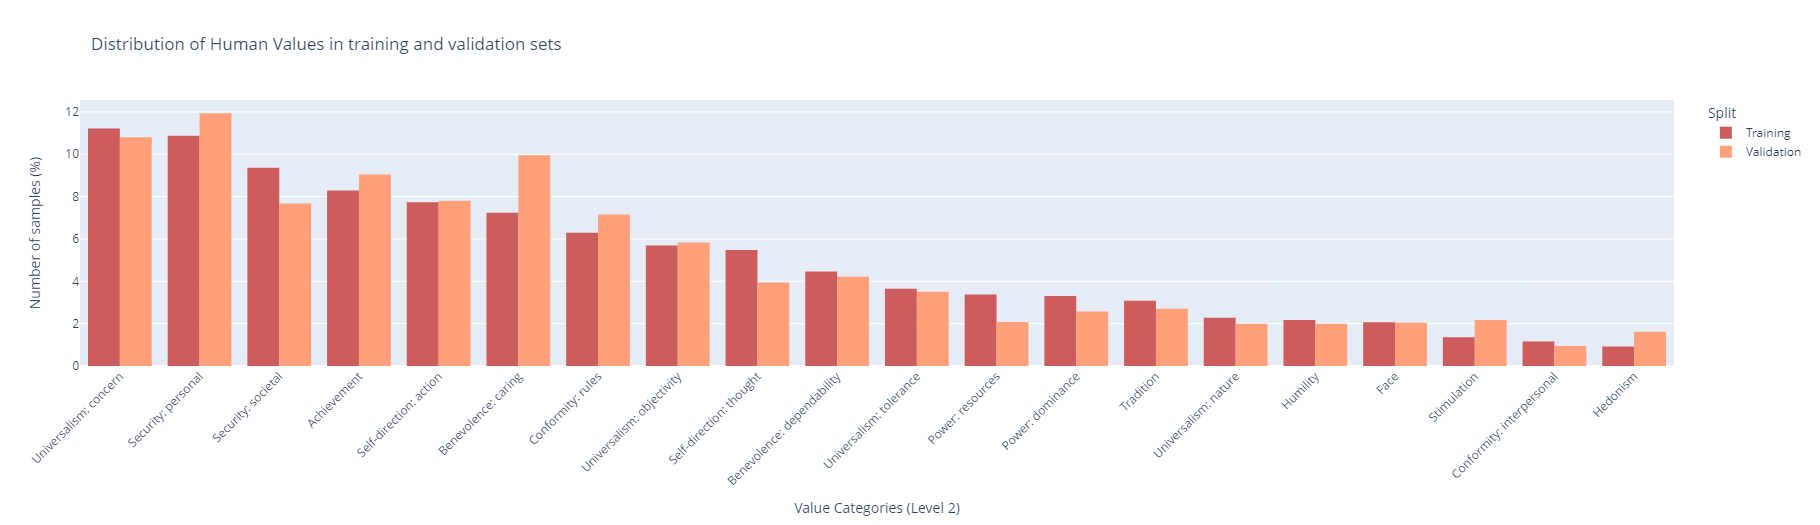
\includegraphics[width=1.\textheight, height=9cm]{figures/label_dist.png}
	\caption{Labels distribution}
	    \label{fig:labels_dist}
	\centering
	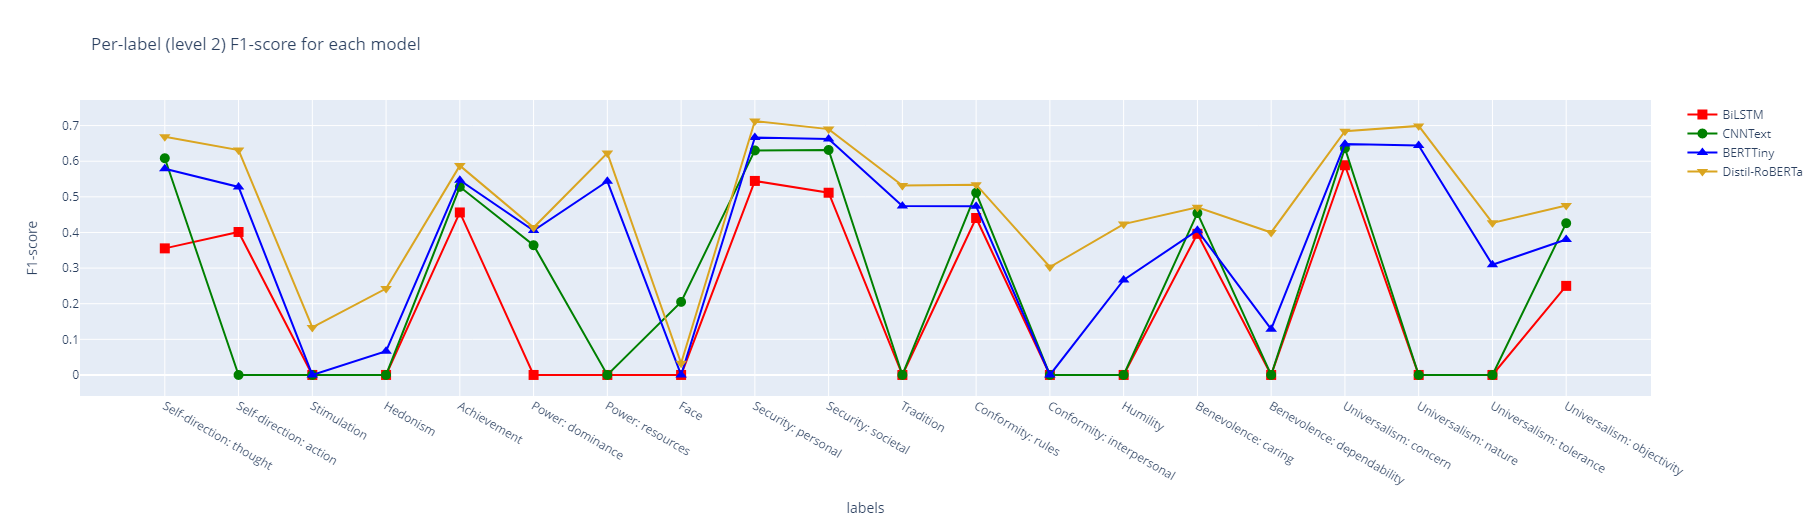
\includegraphics[width=1.\textheight, height=9cm]{figures/models_performance.png}
	\caption{Models performance (F1-Score macro)}
	    \label{fig:models_performance}
\end{sidewaysfigure*}

\attention{DO NOT INSERT CODE IN THIS REPORT}




\bibliography{nlpreport.bib}
\end{document}